% JUMP TO LINE 60, 75
\documentclass[preview, margin=0.6in]{standalone}
\usepackage[letterpaper,portrait,top=0.4in, left=0.6in, right=0.6in, bottom=1in]{geometry}

\usepackage{amsmath, amsfonts, amsthm, amssymb}
\usepackage{graphicx, float}
\usepackage{mathtools}
\usepackage{titlesec}
\usepackage{interval}
\usepackage{hyperref}
\usepackage{siunitx}
\usepackage{titling}
\usepackage{vwcol}
\usepackage{setspace}
\usepackage{empheq}
\usepackage{cancel}
\usepackage{esdiff}
\usepackage{multicol}
\usepackage{mdframed}
\usepackage{esdiff}
\usepackage{tikzsymbols}
\usepackage{multicol}
\usepackage{tikz}
\usepackage{varwidth}
\usepackage{parskip}
\usepackage{pgfplots}
\usetikzlibrary{positioning}
\usetikzlibrary{angles,quotes}
\pgfplotsset{compat=1.18}
\intervalconfig {
	soft open fences
}

\newcommand{\alignedintertext}[1]{%
  \noalign{%
    \vtop{\hsize=\linewidth#1\par
    \expandafter}%
    \expandafter\prevdepth\the\prevdepth
  }%
}

\newtheorem{lemma}{Lemma}

\renewcommand{\qedsymbol}{\Smiley[1.3]}
\newcommand*{\problem}[1]{\section*{Problem #1}}
\newcommand*{\aps}{\section*{AP Corner}}
\newcommand*{\deriv}[1][x]{\ensuremath{\dfrac{\mathrm{d}}{\mathrm{d}#1}}}
\newcommand*{\floor}[1]{\ensuremath{\lfloor #1\rfloor}}
\newcommand*{\lheqzero}{\ensuremath{\underset{\text{L'H}}{\overset{\left[\frac00\right]}{=}}}}
\newcommand*{\lheqinfty}{\ensuremath{\underset{\text{L'H}}{\overset{\left[\frac{\infty}{\infty}\right]}{=}}}}

\DeclareMathOperator{\DNE}{DNE}
\DeclareMathOperator{\sgn}{sgn}

\DeclareMathOperator{\arccsc}{arccsc}
\DeclareMathOperator{\arcsec}{arcsec}
\DeclareMathOperator{\arccot}{arccot}

%opening

\title{\vspace*{-40pt}Problem Set \#62}
\author{Jayden Li}
\date{\today}
% \allowdisplaybreaks
\postdisplaypenalty=100000

\begin{document}
\setstretch{1.25}
\fontsize{12pt}{12pt}\selectfont
\setlength{\abovedisplayskip}{\abovedisplayskip/2}
\setlength{\belowdisplayskip}{\belowdisplayskip/2}
\setlength{\parindent}{0pt}
\setlength{\parskip}{2ex plus 0.5ex minus 0.2ex}
\maketitle

\problem{4}
\begin{center}
	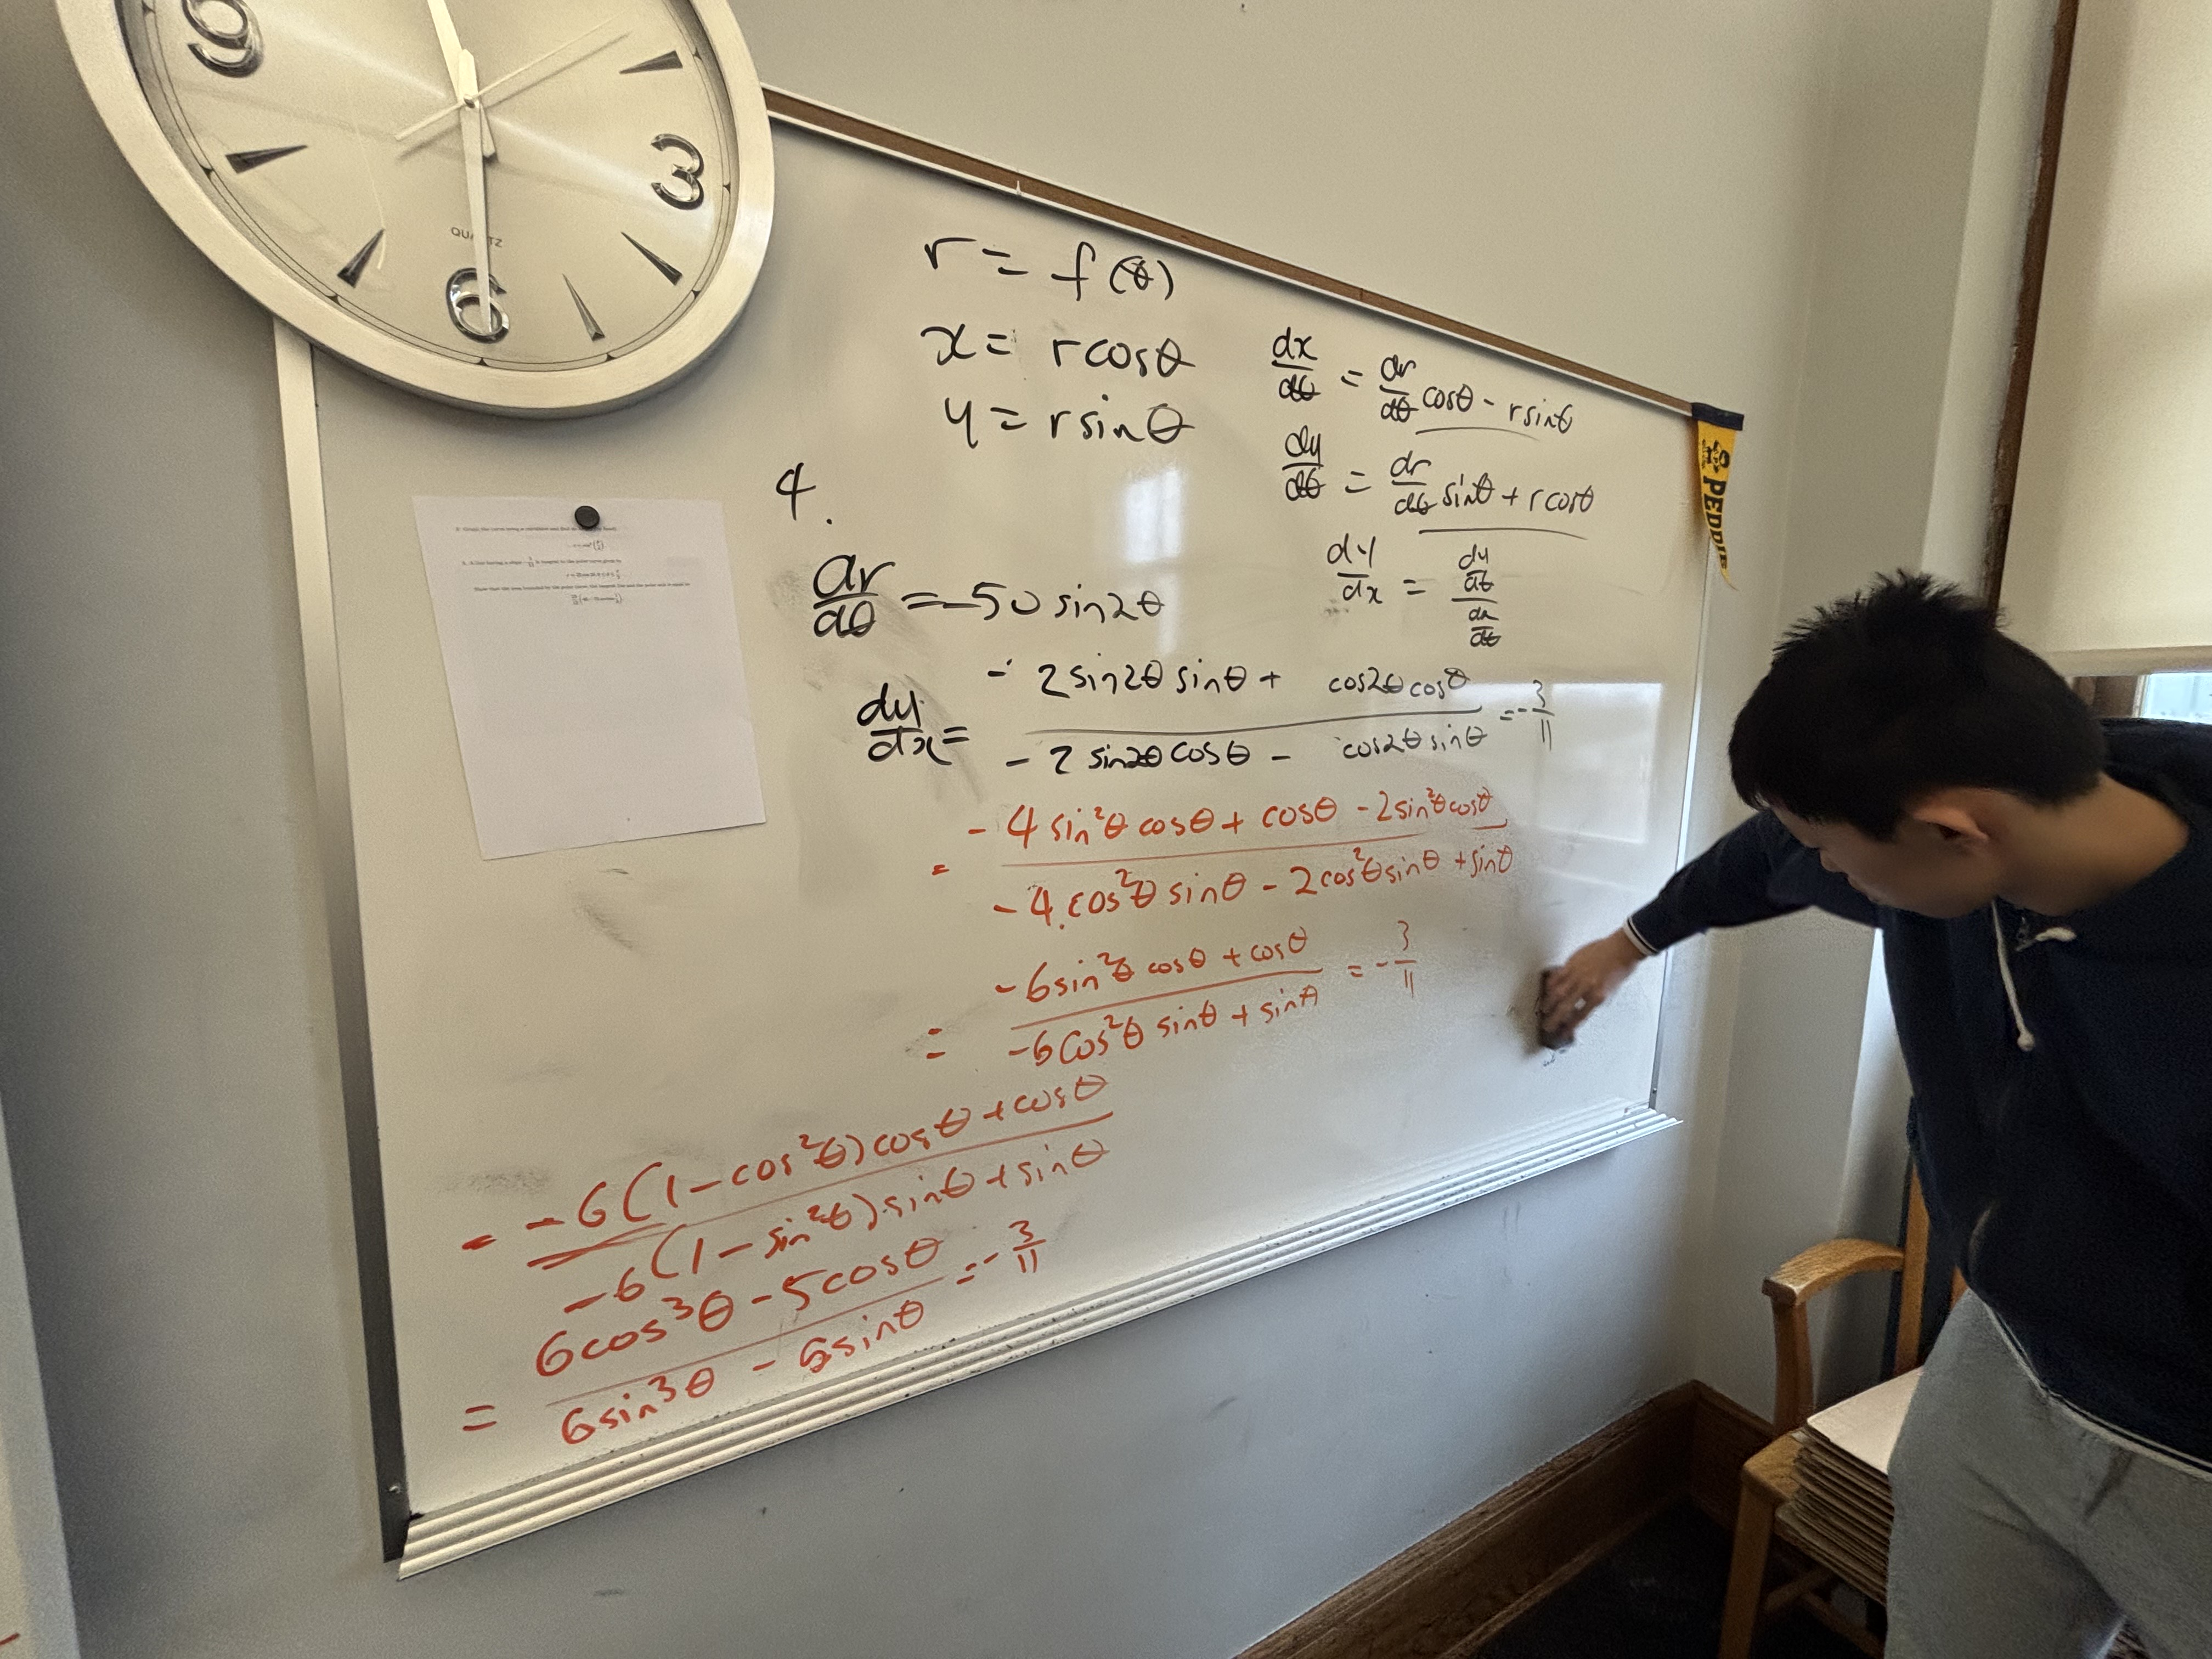
\includegraphics[width=0.9\linewidth]{q4_1.jpeg}
	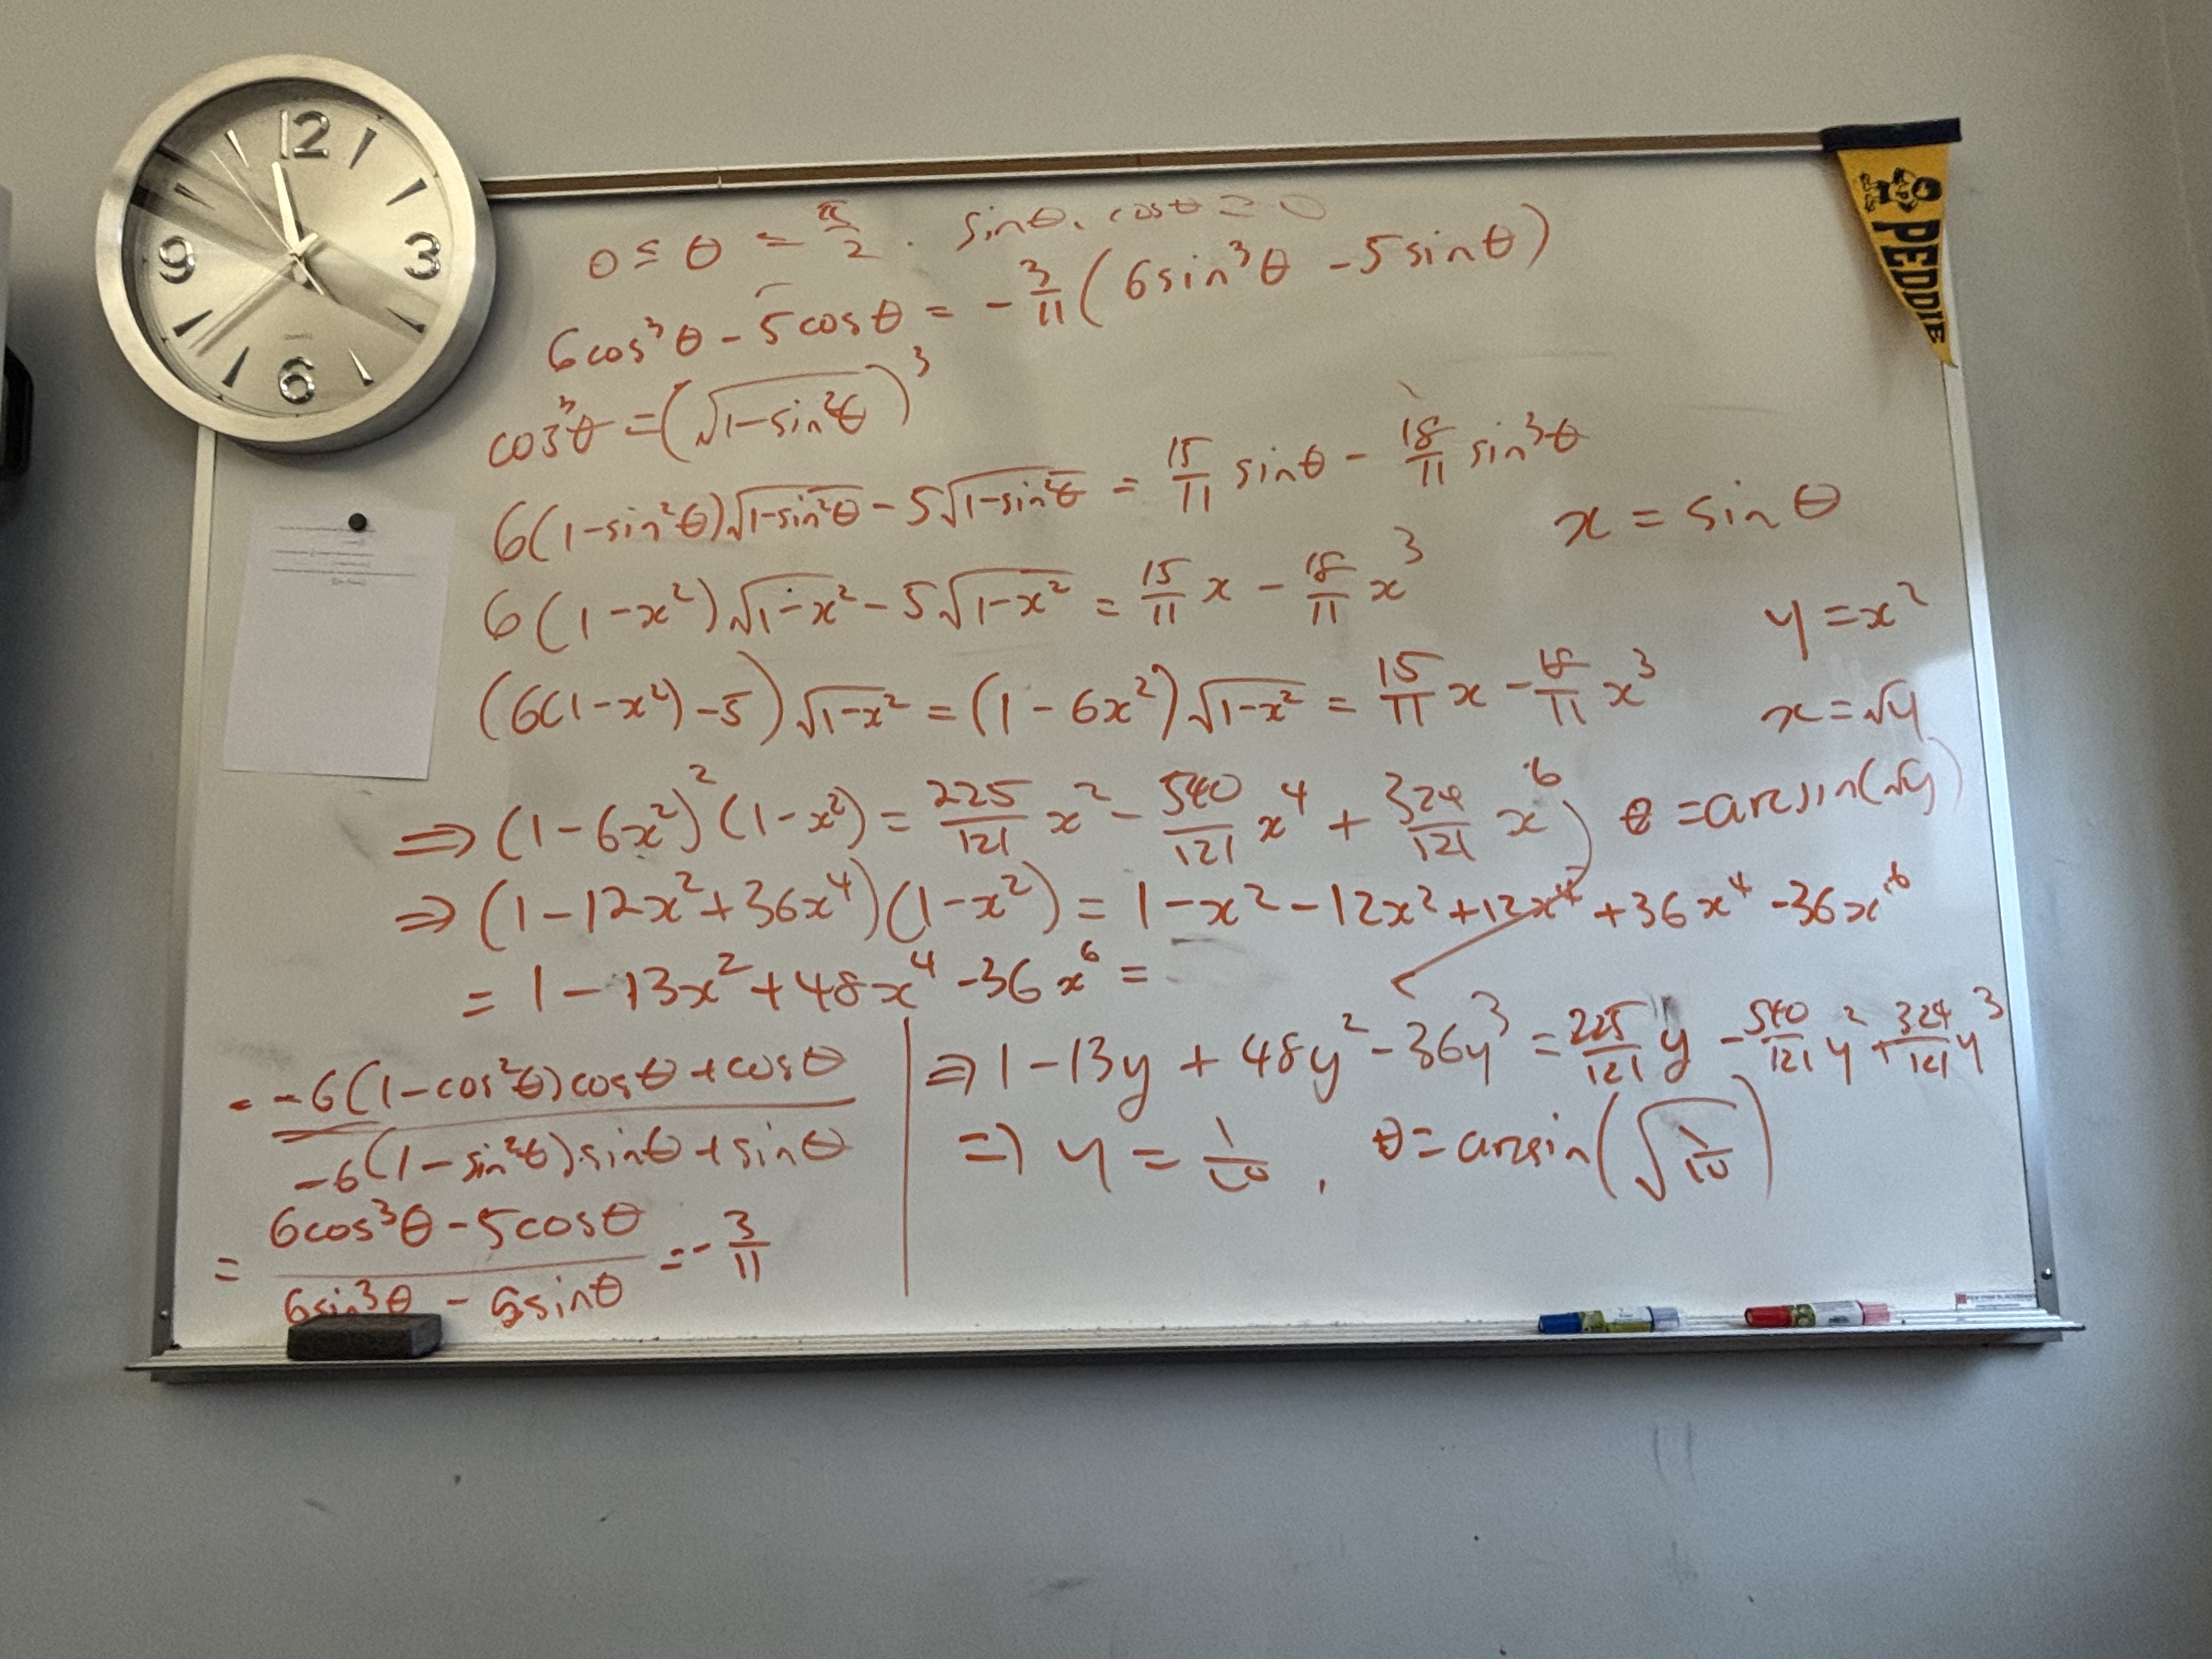
\includegraphics[width=0.9\linewidth]{q4_2.jpeg}
\end{center}

\begin{equation*}
    r=f(\theta)=25\cos2\theta
\end{equation*}

It is known that the slope of the tangent line at $\theta=\varphi=\arcsin \left( \sqrt{1/10 }\right)$ is $-3/11$. Then, we know: 

\hspace{0.6in}$\begin{aligned}[t]
	\sin \varphi
	&=\sqrt{\frac{1}{10}}
	=\frac{1}{\sqrt{10}} \\
	\cos \varphi
	&=\sqrt{1-\left(\sqrt{\frac{1}{10}}\right)^2}
	=\sqrt{1-\frac{1}{10}}
	=\sqrt{\frac{9}{10}}
	=\frac{3}{\sqrt{10}} \\
	\cos 2\varphi
	&=1-2\sin^2\varphi
	=1-2 \left(\sin \varphi\right)^2
	=1-2 \cdot \frac{1}{10}
	=\frac{5}{5}-\frac{1}{5}
	=\frac{4}{5} \\
	\sin 2\varphi 
	&=2\sin \varphi \cos \varphi
	=2\cdot \frac{1}{\sqrt{10}}\cdot \frac{3}{\sqrt{10}}
	=\frac{6}{10}
	=\frac{3}{5}
\end{aligned}$

The coordinates of each point $O,A,B,C$ are known:

\hspace{0.6in}$\begin{aligned}[t]
	O
	&=(0,0) \\
	A
	&=(r\cos \varphi,r\sin\varphi)
	=\left(25\cos2\varphi\cos\varphi,25\cos2\varphi\sin\varphi\right) \\
	&=\left(25 \cdot \frac45 \cdot \frac{3}{\sqrt{10}}, 25\cdot \frac{4}{5}\cdot \frac{1}{\sqrt{10}}\right)
	=\left(\frac{60}{\sqrt{10}}, \frac{20}{\sqrt{10}}\right) \\
	B 
	&=\left(25\cos0\cos0,25\sin0\cos0\right)
	=\left(25,0\right)
\end{aligned}$

From here, we can find the tangent line whose slope is $-3/11$, and passes through point $A$.
\begin{align*}
    y-y_0&=m(x-x_0) \\
	y-\frac{20}{\sqrt{10}}&=-\frac{3}{11}\left(x-\frac{60}{\sqrt{10}}\right)
	\intertext{To find $C$, we need to calculate its polar-axis-intercept, or $x$-intercept:}
	-\frac{20}{\sqrt{10}}\cdot \left(-\frac{11}{3}\right)&=x-\frac{60}{\sqrt{10}} \\
	x&=\frac{220}{3 \sqrt{10}}+\frac{60}{\sqrt{10}}
\end{align*}

Thus, we have $\displaystyle C=\left(\frac{220}{3 \sqrt{10}}+\frac{60}{\sqrt{10}},0\right)$. Knowing the altitude and base of triangle $\triangle OAC$, we can find its area. We can also find the area bound by the polar curve and the polar axis by integration.

\begin{mdframed}
	First, let us find how to represent the arcsine of a number as the arctaengent of another number. Let $\theta=\arcsin x$, then $\sin \theta=x$

	\vspace{-15pt}
	\begin{center}
		\begin{tikzpicture}[
			baseline=(current bounding box.north),
			ang/.style={draw, angle eccentricity=1.5,angle radius=0.6cm}
		]	
			\draw 
			(0,0) coordinate[label=below:{$A$}](A)
		 -- (6,0) coordinate[label=below:{$C$}](C) node[midway,below]{$\sqrt{1-x^2}$}
		 -- (6,3) coordinate[label=above:{$B$}](B) node[midway,right]{$x$}
		 -- cycle node[midway,above,left]{$1$}
			pic["$\theta$",ang]{angle=C--A--B};
		\end{tikzpicture}
	\end{center}

	\begin{equation*}46
		\tan \theta=\frac{x}{\sqrt{1-x^2}}
		\implies\theta=\arctan\left(\frac{x}{\sqrt{1-x^2}}\right)
	\end{equation*}
	\vspace{1pt}
\end{mdframed}

\hspace{0.6in}$\begin{aligned}[t]
	S_{OAC}
	&=\frac12 \left(\frac{220}{3 \sqrt{10}}+\frac{60}{\sqrt{10}}\right) \left(\frac{20}{\sqrt{10}}\right)
	=\frac12 \left(\frac{4400}{30}+\frac{1200}{10}\right)
	=\frac{220}{3}+\frac{180}{3}
	=\frac{400}{3} \\
	S_{OAB}
	&=\frac12 \int_{0}^{\varphi}\left(f(\theta)\right)^2\,\mathrm{d}\theta
	=\frac12 \int_{0}^{\varphi}\left(25\cos2\theta\right)^2\,\mathrm{d}\theta
	=\frac{625}{2}\int_{0}^{\varphi}\cos^22\theta\,\mathrm{d}\theta
	=\frac{625}{2}\int_{0}^{\varphi}\frac{1+\cos4\theta}{2}\,\mathrm{d}\theta \\
	&=\frac{625}{4}\left[\theta+\frac{\sin4\theta}{4}\right]_{0}^{\varphi}
	=\frac{625}{4}\left(\varphi+\frac14 \sin 4\varphi\right)
	=\frac{625}{4}\left(\varphi+\frac12 \sin 2\varphi \cos 2\varphi\right) \\
	&=\frac{625}{4}\left(\varphi+\frac12 \cdot \frac{4}{5}\cdot \frac{3}{5}\right)
	=\frac{625}{4}\left(\arcsin \sqrt{\frac{1}{10}}+\frac{6}{25}\right)
	=\frac{625}{4}\left(\arctan\left(\frac{\sqrt{\frac{1}{10}}}{\sqrt{1-\frac{1}{10}}}\right)+\frac{6}{25}\right) \\
	&=\frac{625}{4}\left(\arctan\left(\frac{\frac{1}{\sqrt{10}}}{\frac{3}{\sqrt{10}}}\right)+\frac{6}{25}\right)
	=\frac{625}{4}\left(\arctan\left(\frac13\right)+\frac{6}{25}\right) \\
	\alignedintertext{\hspace{-0.6in}Then we can subtract these two areas, as in the diagram, to obtain the desired area.}
	S_{ABC}
	&=S_{OAC}-S_{OAB}
	=\frac{400}{3}-\frac{625}{4}\left(\arctan\left(\frac13\right)+\frac{6}{25}\right)
	=\frac{400}{3}-\frac{625}{4}\arctan\frac13-\frac{25\cdot 3}{2} \\
	&=\frac{800}{6}-\frac{225}{6}-\frac{625}{4}\arctan\frac13
	=\frac{575}{6}-\frac{625}{4}\arctan\frac13
	=\frac{25}{12}\cdot 46-\frac{25}{12}\cdot 75 \arctan \frac13 \\
	&=\boxed{\frac{25}{12}\left(46-75\arctan \frac13\right)}
\end{aligned}$

\end{document}
